\section{\textsc{Egg pancakes}}

\subsection*{Ingredients for 2 portions:}

\begin{tabular}{p{7.5cm} p{7.5cm}}
	& \\
	100g flour & 40g sugar \\
	300ml milk & 4 eggs \\
	pinch of salt & oil for the pan \\
	\multicolumn{2}{l}{Icing sugar for decoration}
\end{tabular}

\subsection*{Serving suggestion:}

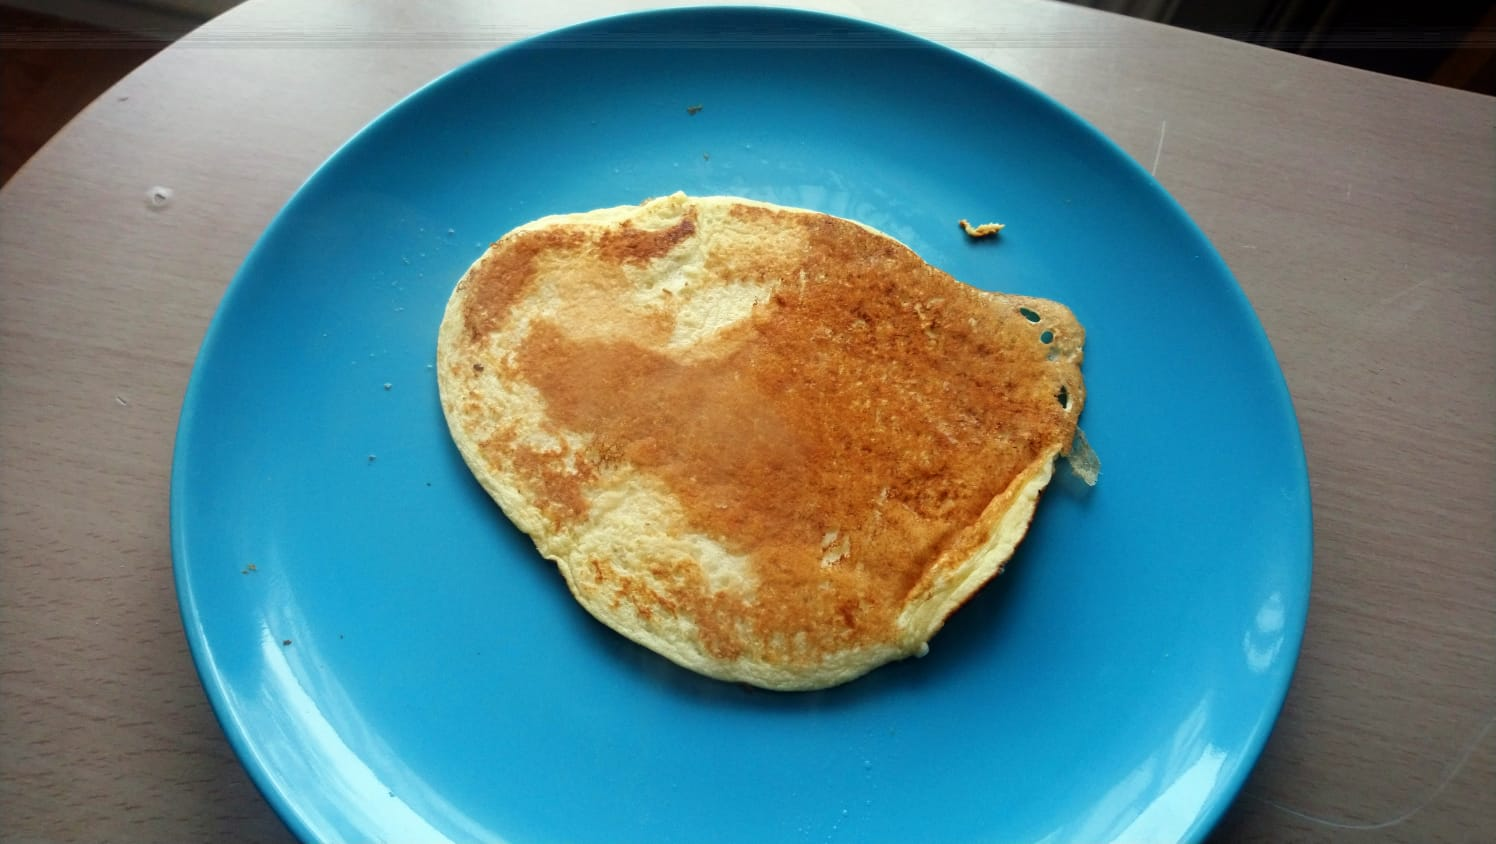
\includegraphics[width=\textwidth]{img/pancakes/pancakes_gebraten.jpg} \cite{pancakes}

\subsection*{How it's done:}

\begin{tabular}{p{15cm}}
	\\
  Separate the eggs and whisk the egg whites with a whisk.\\
  Mix the sugar, milk, egg yolk and pinch of salt.\\
  Sift the flour into the mixture. This makes the dough finer.\\
  Now fold in the beaten egg white slowly and carefully so that it does not disintegrate again.\\
  Heat the oil in a pan. To check, hold the back of a wooden cooking spoon or a wooden stick in the oil. If the oil blows, it's hot enough.\\
  Pour the dough into the pan with a medium ladle.\\
  Brown the pancakes on both sides until golden brown.\\
  Sprinkle with icing sugar and serve hot.
\end{tabular}
